%!TEX program = xelatex
% ==============================================================================
% AA CONFIGURAZIONE DI BASE ED ENGINE
% ==============================================================================
% BB CLASSE DEL DOCUMENTO
\documentclass[11pt, a4paper]{article}

% ==============================================================================
% AA LINGUA, FONT E TIPOGRAFIA
% ==============================================================================
% BB GESTIONE FONT XELATEX
\usepackage{fontspec}
\setmainfont{Latin Modern Roman}

% BB LOCALIZZAZIONE LINGUISTICA
\usepackage[italian]{babel}

% BB TIPOGRAFIA E MICRO-ESTENSIONI
\usepackage[protrusion=true]{microtype}
\raggedbottom

% ==============================================================================
% AA LAYOUT DI PAGINA E SPAZIATURA PARAGRAFI
% ==============================================================================
% BB GEOMETRIA DEI MARGINI
\usepackage[left=2.4cm, right=1.35cm, top=2cm, bottom=2cm]{geometry}

% BB CONTROLLO SPAZIATURA TRA PARAGRAFI
\usepackage[skip=3pt plus 1pt minus 1pt]{parskip}

% ==============================================================================
% AA MOTORE DEI COLORI E MACRO LOCALI
% ==============================================================================
% BB CARICAMENTO CORE XCOLOR IN SPAZIO GRAY PURO
\usepackage[gray]{xcolor}

% ==============================================================================
% AA MATEMATICA E SIMBOLI SCIENTIFICI
% ==============================================================================
% BB PACCHETTI MATEMATICI UNICODE
\usepackage{mathtools}
\usepackage[warnings-off={mathtools-overbracket,mathtools-colon}]{unicode-math}
\setmathfont{Latin Modern Math}

% BB METRICHE MATRICI E FORMULE DISPLAY
\setlength{\arraycolsep}{10pt}
\setlength{\abovedisplayskip}{3pt plus 1pt minus 1pt}
\setlength{\belowdisplayskip}{3pt plus 1pt minus 1pt}
\setlength{\abovedisplayshortskip}{0pt plus 1pt}
\setlength{\belowdisplayshortskip}{2pt plus 1pt minus 1pt}
\allowdisplaybreaks

% ==============================================================================
% AA GRAFICA ED ELEMENTI FLOTTANTI
% ==============================================================================
% BB MOTORE DI INCLUSIONE GRAFICA E GESTIONE RIGIDA
\usepackage{graphicx}
\graphicspath{{./E5_Images/}}
\usepackage{float}

% ==============================================================================
% AA TITOLI E STRUTTURA DEL DOCUMENTO (MONOCROMATICI NERI)
% ==============================================================================
% BB PACCHETTO TITLESEC
\usepackage{titlesec}

% BB FORMATTAZIONE TIPOGRAFICA (TITOLI NERI)
\titleformat{\section}{\normalfont\Large\bfseries}{\thesection}{1em}{}
\titleformat{name=\section,numberless}{\normalfont\Large\bfseries}{}{0pt}{}
\titleformat{\subsection}{\normalfont\large\bfseries}{\thesubsection}{1em}{}
\titleformat{name=\subsection,numberless}{\normalfont\large\bfseries}{}{0pt}{}
\titleformat{\subsubsection}{\normalfont\normalsize\bfseries}{\thesubsubsection}{1em}{}
\titleformat{name=\subsubsection,numberless}{\normalfont\normalsize\bfseries}{}{0pt}{}

% BB SPAZIATURA VERTICALE DEI TITOLI
\titlespacing*{\section}{0pt}{1.2ex plus 0.4ex minus 0.2ex}{0.6ex plus 0.2ex}
\titlespacing*{\subsection}{0pt}{1ex plus 0.3ex minus 0.2ex}{0.5ex plus 0.2ex}
\titlespacing*{\subsubsection}{0pt}{0.8ex plus 0.2ex minus 0.1ex}{0.4ex plus 0.1ex}

% ==============================================================================
% AA INTEGRAZIONE AMBIENTE MATLAB
% ==============================================================================
% BB CARICAMENTO PACCHETTO MATLAB
\usepackage{matlab}

% BB ATTIVAZIONE SEGNALIBRI E INDICE MATLAB
\matlabmultipletitles
\matlabhastoc

% ==============================================================================
% AA IPERTESTO, SEGNALIBRI ED ELENCHI
% ==============================================================================
% BB CONFIGURAZIONE HYPERREF E METADATI PDF
\hypersetup{
    hidelinks,
    pdfauthor={Francesco Lo Verde},
    pdftitle={Cinematica inversa spazi operativi manipolatore RRR}
}

% BB SEGNALIBRI AVANZATI
\usepackage{bookmark}

% BB FORMATTAZIONE ELENCHI PUNTATI E NUMERATI
\usepackage{enumitem}
\setlist{itemsep=3.5pt plus 1pt minus 1pt, topsep=4pt plus 1pt minus 1pt, partopsep=0pt, parsep=1pt}

\begin{document}
\matlabtitle{Cinematica inversa e spazi operativi manipolatore planare RRR}

\begin{par}
\begin{center}
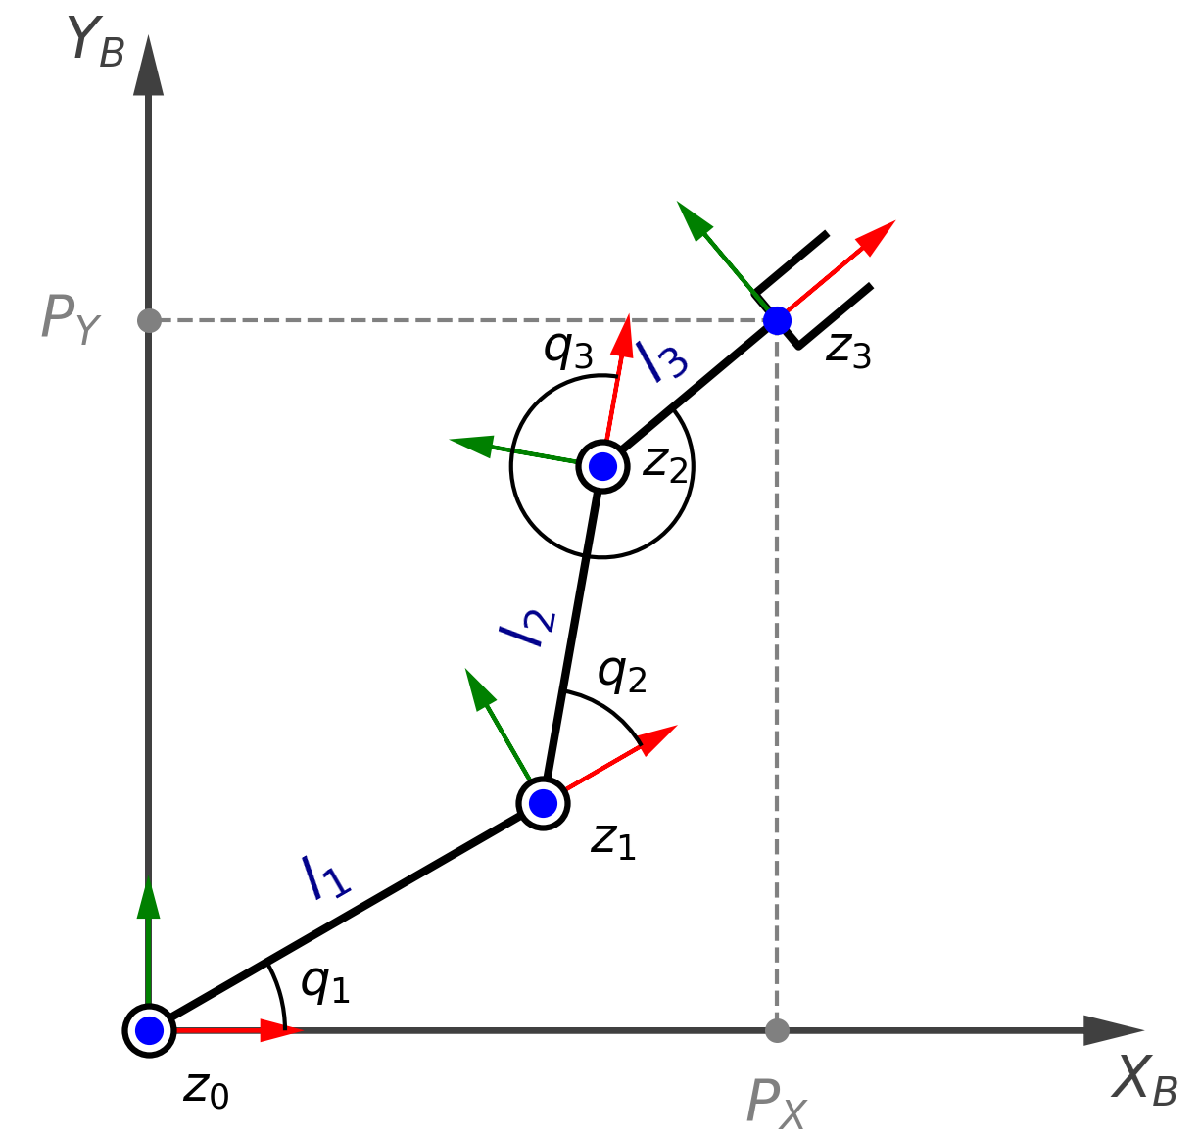
\includegraphics[width=0.45\linewidth]{image_0}
\end{center}
\end{par}

\begin{par}
\begin{flushleft}
Un \textbf{manipolatore RRR} planare è un braccio robotico composto da tre giunti rotoidali i cui assi di rotazione sono tutti paralleli. Questo tipo di robot opera su un piano e possiede \textit{3 gradi di libertà} (\textbf{DoF}).
\end{flushleft}
\end{par}

\begin{par}
\begin{flushleft}
Lo \textbf{spazio operativo} descrive la posa dell'organo terminale (\textit{end-effector}). Per un manipolatore RRR planare, la posa è definita da due coordinate cartesiane $(P_x ,P_y )$ e un orientamento $\phi$ rispetto a un asse fisso. Lo spazio operativo ha quindi dimensione $m=3$ ed è descritto dal vettore:
\end{flushleft}
\end{par}
\[
    \mathbf{r} =
    \begin{pmatrix}
        P_x \\
        P_y \\
        \phi
    \end{pmatrix}
\]
\begin{par}
\begin{flushleft}
Poiché il numero di gradi di libertà ($n=3$) è uguale alla dimensione dello spazio operativo ($m=3$), il manipolatore è in grado di controllare in modo indipendente sia la posizione che l'orientamento del suo end-effector. Questo gli permette di raggiungere (quasi) ogni posa desiderata all'interno del suo spazio di lavoro.
\end{flushleft}
\end{par}

\matlabheading{Cinematica diretta manipolatore planare RRR}

\begin{par}
\begin{flushleft}
Per risolvere il problema analiticamente, si utilizza il \textit{Symbolic Math Toolbox}. Si definiscono prima di tutto le variabili simboliche che rappresentano le costanti del sistema (\textbf{le lunghezze dei bracci}) e le variabili (\textbf{gli angoli dei giunti} e la \textbf{posa desiderata}).
\end{flushleft}
\end{par}

\begin{matlabcode}
clc; clear; close all;

% l1, l2, l3 sono le lunghezze dei tre bracci del manipolatore.
syms l1 l2 l3 real;

% q1, q2, q3_calc sono gli angoli dei tre giunti rotoidali.
syms q1 q2 q3_calc real;

% Px, Py, phi rappresentano la posizione (x, y) e l'orientamento desiderati.
syms Px Py phi real;

% P_wx, P_wy rappresentano la posizione del polso
syms P_wx P_wy real;
\end{matlabcode}

\begin{par}
\begin{flushleft}
La cinematica diretta calcola la posizione $(x,y)$ e l'orientamento $\phi$ dell'end-effector a partire dagli angoli di giunto $(q_1 ,q_2 ,q_3 )$ noti.
\end{flushleft}
\end{par}
\newpage
\begin{matlabcode}
% Posizione primo giunto (origine)
x0 = 0;
y0 = 0;
% Posizione secondo giunto (Z1)
x1 = x0 + l1 * cos(q1);
y1 = y0 + l1 * sin(q1);
% Posizione terzo giunto (Z2)
x2 = x1 + l2 * cos(q1 + q2);
y2 = y1 + l2 * sin(q1 + q2);
% Posizione end-effector (Z3)
px_calc = x2 + l3 * cos(q1 + q2 + q3_calc);
py_calc = y2 + l3 * sin(q1 + q2 + q3_calc);

fprintf('Equazioni cinematica diretta (posizione):\n');
fprintf('Px = %s\n', px_calc);
fprintf('Py = %s\n', py_calc);
\end{matlabcode}
\begin{matlaboutput}
Equazioni cinematica diretta (posizione):
\end{matlaboutput}
\begin{matlaboutput}
Px = l2*cos(q1 + q2) + l1*cos(q1) + l3*cos(q1 + q2 + q3_calc)
\end{matlaboutput}
\begin{matlaboutput}
Py = l2*sin(q1 + q2) + l1*sin(q1) + l3*sin(q1 + q2 + q3_calc)
\end{matlaboutput}

\begin{par}
\begin{flushleft}
 L'orientamento dell'end-effector $\phi$ è dato dalla somma degli angoli dei giunti
\end{flushleft}
\end{par}

\begin{matlabcode}
% phi_calc per non confonderlo con phi
phi_calc = q1 + q2 + q3_calc;
fprintf('Phi = %s\n', phi_calc);
\end{matlabcode}
\begin{matlaboutput}
Phi = q1 + q2 + q3_calc
\end{matlaboutput}

\matlabheading{Cinematica inversa manipolatore planare RRR}

\begin{par}
\begin{flushleft}
La \textbf{cinematica inversa} si occupa di determinare il vettore degli angoli dei giunti $\mathbf{q}={\bigl\lbrack q_1 \;\;q_2 \;\;q_3 \bigr\rbrack }^T$ che permette all'end-effector di raggiungere una \textbf{posa desiderata}, data dal vettore $\mathbf{r}={\bigl\lbrack P_x \;\;P_y \;\;\phi \bigr\rbrack }^T$.
\end{flushleft}
\end{par}

\begin{par}
\begin{flushleft}
In altre parole, data una specifica posizione ($P_x ,P_y$) e un orientamento $\phi$ nello spazio operativo, l'obiettivo è trovare la configurazione dei giunti che realizzi quella posa.
\end{flushleft}
\end{par}

\begin{par}
\begin{flushleft}
A differenza della cinematica diretta, che ammette sempre una soluzione unica, il problema inverso è più complesso e può avere:
\end{flushleft}
\end{par}

\begin{par}
\begin{flushleft}
\textbf{Nessuna soluzione:} se la posa è fuori dallo spazio di lavoro del robot.
\end{flushleft}
\end{par}

\begin{par}
\begin{flushleft}
\textbf{Una o più soluzioni:} diverse configurazioni dei giunti portano alla stessa posa dell'end-effector.
\end{flushleft}
\end{par}

\begin{par}
\begin{flushleft}
La posizione finale desiderata dell'end-effector $(P_x ,P_y )$ è una funzione complessa e accoppiata di tutti e tre gli angoli $(q_1 ,q_2 ,q_3 )$. Tentare di risolvere direttamente il sistema sarebbe estremamente difficile. L'informazione cruciale che permette di sbloccare il problema è l'\textbf{orientamento finale}, cioè $\phi =q_1 +q_2 +q_3$. La conoscenza della \textbf{posizione} dell'\textbf{end-effector} $(x,y)$, del suo \textbf{orientamento} $\phi$ e della \textbf{lunghezza} dell'ultimo \textbf{braccio} $l_3$, permette di calcolare \textit{univocamente} la posizione del giunto precedente (il "polso"), indicata con $(P_{wx} ,P_{wy} )$.
\end{flushleft}
\end{par}

\begin{par}
\begin{flushleft}
La posizione dell'end-effector $(P_x ,P_y )$ può essere vista come la somma vettoriale della posizione del polso, indicata con $P_w =(P_{wx} ,P_{wy} )$, e del vettore corrispondente al terzo braccio:
\end{flushleft}
\end{par}
\[
    \begin{pmatrix}
        P_x \\
        P_y
    \end{pmatrix}
    =
    \begin{pmatrix}
        P_{wx} \\
        P_{wy}
    \end{pmatrix}
    + \mathbf{R}(\phi )
    \begin{pmatrix}
        l_{3}\\
        0
    \end{pmatrix}
\]
\begin{par}
\begin{flushleft}
Dove:
\end{flushleft}
\end{par}

\begin{par}
\begin{flushleft}
Il vettore $\left(\begin{array}{c}
l_3 \\
0
\end{array}\right)$ rappresenta il vettore del link $3$ descritto nel suo sistema di riferimento locale, in cui l'asse $x$ è allineato con la direzione del link stesso.
\end{flushleft}
\end{par}
\newpage
\begin{par}
\begin{flushleft}
La matrice $\mathbf{R}(\phi )$ è la matrice di rotazione associata all'orientamento finale $\phi$. Isolando la posizione del polso $P_w$, si ottiene:
\end{flushleft}
\end{par}
\[
    \begin{pmatrix}
        P_{wx} \\
        P_{wy}
    \end{pmatrix}
    =
    \begin{pmatrix}
        P_x \\
        P_y
    \end{pmatrix}
    - \mathbf{R}(\phi )
    \begin{pmatrix}
        l_{3}\\
        0
    \end{pmatrix}
    \qquad\longrightarrow\qquad
    \begin{pmatrix}
        P_{wx} \\
        P_{wy}
    \end{pmatrix}
    =
    \begin{pmatrix}
        P_x \\
        P_y
    \end{pmatrix}
    -
    \begin{pmatrix}
        \cos(\phi) & -\sin(\phi) \\
        \sin(\phi) & \cos(\phi)
    \end{pmatrix}
    \begin{pmatrix}
        l_{3}\\
        0
    \end{pmatrix}
\]
\[
    \begin{pmatrix}
        P_{wx} \\
        P_{wy}
    \end{pmatrix}
    =
    \begin{pmatrix}
        P_x \\
        P_y
    \end{pmatrix}
    -
    \begin{pmatrix}
        l_{3}\cos(\phi)\\
        l_{3}\sin(\phi)
    \end{pmatrix}
\]
\begin{matlabcode}
% Matrice R(phi)
R = [cos(phi) -sin(phi); sin(phi) cos(phi)];

fprintf('Matrice R:\n');
disp(R);
\end{matlabcode}
\begin{matlaboutput}
Matrice R:
\end{matlaboutput}

\begin{matlabsymbolicoutput}
$\displaystyle \left(\begin{array}{cc}
\cos \left(\phi \right) & -\sin \left(\phi \right)\\
\sin \left(\phi \right) & \cos \left(\phi \right)
\end{array}\right)$
\end{matlabsymbolicoutput}

\begin{matlabcode}
% Vettore link 3
l3_vec = [l3; 0];

% Vettore posizione end-effector
Pe_calc = [px_calc; py_calc];
fprintf('Posizione end-effector:\n');
disp(Pe_calc);
\end{matlabcode}
\begin{matlaboutput}
Posizione end-effector:
\end{matlaboutput}
\begin{matlabsymbolicoutput}
$\displaystyle \left(\begin{array}{c}
l_2 \,\cos \left(q_1 +q_2 \right)+l_1 \,\cos \left(q_1 \right)+l_3 \,\cos \left(q_1 +q_2 +q_{3,\textrm{calc}} \right)\\
l_2 \,\sin \left(q_1 +q_2 \right)+l_1 \,\sin \left(q_1 \right)+l_3 \,\sin \left(q_1 +q_2 +q_{3,\textrm{calc}} \right)
\end{array}\right)$
\end{matlabsymbolicoutput}
\begin{matlabcode}

% Posizione polso
Pe = [Px; Py];
fprintf('Posizione polso:\n');
Pw_des = Pe - R * l3_vec;
disp(Pw_des);
\end{matlabcode}
\begin{matlaboutput}
Posizione polso:
\end{matlaboutput}
\begin{matlabsymbolicoutput}
$\displaystyle \left(\begin{array}{c}
\textrm{Px}-l_3 \,\cos \left(\phi \right)\\
\textrm{Py}-l_3 \,\sin \left(\phi \right)
\end{array}\right)$
\end{matlabsymbolicoutput}

\begin{par}
\begin{flushleft}
A questo punto, è fondamentale verificare la \textbf{raggiungibilità} del polso. La posizione $P_w$ deve trovarsi all'interno dello spazio di lavoro del "\textit{sotto-manipolatore}" RR formato dai primi due bracci. La sua distanza dall'origine, $\sqrt{P_{wx}^2 +P_{wy}^2 }$, deve essere compresa tra l'estensione minima e massima dei bracci $l_1$ e $l_2$:
\end{flushleft}
\end{par}

\[
    |l_1 -l_2 |\le \sqrt{P_{wx}^2 +P_{wy}^2 }\le l_1 +l_2
\]

\begin{par}
\begin{flushleft}
Se questa \textbf{condizione} è \textbf{soddisfatta}, il punto $P_w = (P_{wx}, P_{wy})$ è all'interno dello spazio di lavoro del manipolatore RR. Questo garantisce che esista una soluzione reale per gli angoli $q_1$ e $q_2$. Matematicamente, questo assicura che il valore $\cos (q_2 )$ sarà compreso nell'intervallo $[-1,1]$.
\end{flushleft}
\end{par}

\begin{par}
\begin{flushleft}
Se questa \textbf{condizione non} è \textbf{soddisfatta}, la posa desiderata è irraggiungibile. Cioè, non esiste alcuna configurazione reale degli angoli $q_1$ e $q_2$ che possa posizionare il polso in quel punto. Il valore di $\cos (q_2 )$ avrebbe modulo maggiore di $1$, rendendo impossibile trovare un angolo reale $q_2$.
\end{flushleft}
\end{par}

\begin{par}
\begin{flushleft}
Si devono quindi trovare $q_1$ e $q_2$ tali che il manipolatore RR posizioni il suo estremo in $P_w$.
\end{flushleft}
\end{par}
\newpage
\matlabheadingtwo{Calcolo variabile di giunto \texorpdfstring{$q_2$}{q2}}

\begin{par}
\begin{flushleft}
Le equazioni di cinematica diretta per il polso sono:
\end{flushleft}
\end{par}

\[
\begin{aligned}
    P_{wx} &= l_1 \cos(q_1) + l_2 \cos(q_1 + q_2) \\
    P_{wy} &= l_1 \sin(q_1) + l_2 \sin(q_1 + q_2)
\end{aligned}
\]

\begin{par}
\begin{flushleft}
Per trovare $q_2$, si elevano al quadrato e si sommano le due equazioni.
\end{flushleft}
\end{par}

\begin{matlabcode}
Pw = simplify(subs(Pe_calc, q3_calc, phi - q1 - q2) - (R * l3_vec));
fprintf('P_{wx}^2 + P_{wy}^2 = \n');
quadSum = Pw(1)^2 + Pw(2)^2;
quadSum = simplify(quadSum);
disp(quadSum);
\end{matlabcode}
\begin{matlaboutput}
P_{wx}^2 + P_{wy}^2 =
\end{matlaboutput}
\begin{matlabsymbolicoutput}
$\displaystyle {l_1 }^2 +2\,\cos \left(q_2 \right)\,l_1 \,l_2 +{l_2 }^2 $
\end{matlabsymbolicoutput}

\begin{matlabcode}

eq = P_wx^2 + P_wy^2 == quadSum;
cos_q2 = isolate(eq, cos(q2));
fprintf('Equazione simbolica cos(q2):\n');
disp(cos_q2);
\end{matlabcode}
\begin{matlaboutput}
Equazione simbolica cos(q2):
\end{matlaboutput}
\begin{matlabsymbolicoutput}
$\displaystyle \cos \left(q_2 \right)=\frac{{P_{\textrm{wx}} }^2 +{P_{\textrm{wy}} }^2 -{l_1 }^2 -{l_2 }^2 }{2\,l_1 \,l_2 }$
\end{matlabsymbolicoutput}
\begin{matlabcode}

% Avendo i valori numerici
% Pw_calc = Pe_calc - (R * l3_vec);
% eq_calc = Pw_calc(1)^2 + Pw_calc(2)^2 == quadSum;
% sol_cos_q2_calc = isolate(eq_calc, cos(q2));
% disp(sol_cos_q2_calc);
\end{matlabcode}

\begin{par}
\begin{flushleft}
Poiché $\sin^2 (q_2 )+\cos^2 (q_2 )=1$, si hanno due possibili soluzioni per $\sin (q_2 )$:
\end{flushleft}
\end{par}

\[
    \sin(q_2) = \pm \sqrt{1 - \cos(q_2)^2}
\]

\begin{par}
\begin{flushleft}
Queste due soluzioni corrispondono a due diverse configurazioni del braccio:
\end{flushleft}
\end{par}

\begin{itemize}
\setlength{\itemsep}{-1ex}
   \item{\begin{flushleft} \textbf{Gomito basso} (soluzione positiva): il gomito è sotto la linea che collega la base al polso $P_w$ \end{flushleft}}
   \item{\begin{flushleft} \textbf{Gomito alto} (soluzione negativa): il gomito è sopra la linea che collega la base al polso $P_w$ \end{flushleft}}
\end{itemize}

\begin{par}
\begin{flushleft}
L'angolo $q_2$ si trova quindi con:
\end{flushleft}
\end{par}

\[
    q_2 = \textrm{atan2}(\sin(q_2), \cos(q_2))
\]


\begin{matlabcode}
cos_q2_val = rhs(cos_q2);
sin_q2_pos = sqrt(1 - cos_q2_val^2);
sin_q2_neg = -sqrt(1 - cos_q2_val^2);
q2_neg = atan2(sin_q2_neg, cos_q2_val);
q2_pos = atan2(sin_q2_pos, cos_q2_val);
fprintf('Valore q2 per valore seno negativo:\n');
disp(q2_neg);
\end{matlabcode}
\begin{matlaboutput}
Valore q2 per valore seno negativo:
\end{matlaboutput}
\begin{matlabsymbolicoutput}
$\displaystyle \textrm{atan2}\left(-2\,\sqrt{1-\frac{{{\left({P_{\textrm{wx}} }^2 +{P_{\textrm{wy}} }^2 -{l_1 }^2 -{l_2 }^2 \right)}}^2 }{4\,{l_1 }^2 \,{l_2 }^2 }},\frac{{P_{\textrm{wx}} }^2 +{P_{\textrm{wy}} }^2 -{l_1 }^2 -{l_2 }^2 }{l_1 \,l_2 }\right)$
\end{matlabsymbolicoutput}
\begin{matlabcode}
fprintf('Valore q2 per valore seno positivo:\n');
disp(q2_pos);
\end{matlabcode}
\begin{matlaboutput}
Valore q2 per valore seno positivo:
\end{matlaboutput}
\begin{matlabsymbolicoutput}
$\displaystyle \textrm{atan2}\left(2\,\sqrt{1-\frac{{{\left({P_{\textrm{wx}} }^2 +{P_{\textrm{wy}} }^2 -{l_1 }^2 -{l_2 }^2 \right)}}^2 }{4\,{l_1 }^2 \,{l_2 }^2 }},\frac{{P_{\textrm{wx}} }^2 +{P_{\textrm{wy}} }^2 -{l_1 }^2 -{l_2 }^2 }{l_1 \,l_2 }\right)$
\end{matlabsymbolicoutput}

\matlabheadingtwo{Calcolo variabile di giunto \texorpdfstring{$q_1$}{q1}}

\begin{par}
\begin{flushleft}
Una volta noto $q_2$, si può risolvere per $q_1$. Il sistema di equazioni per la posizione del polso può essere riscritto come un sistema lineare nelle incognite $\cos (q_1 )$ e $\sin (q_1 )$
\end{flushleft}
\end{par}

\begin{matlabcode}
eq_Pwx = P_wx == Pw(1);
eq_Pwy = P_wy == Pw(2);

fprintf('Equazione P_wx:\n');
disp(eq_Pwx);
\end{matlabcode}
\begin{matlaboutput}
Equazione P_wx:
\end{matlaboutput}
\begin{matlabsymbolicoutput}
$\displaystyle P_{\textrm{wx}} =l_2 \,\cos \left(q_1 +q_2 \right)+l_1 \,\cos \left(q_1 \right)$
\end{matlabsymbolicoutput}
\begin{matlabcode}
fprintf('Equazione P_wy:\n');
disp(eq_Pwy);
\end{matlabcode}
\begin{matlaboutput}
Equazione P_wy:
\end{matlaboutput}
\begin{matlabsymbolicoutput}
$\displaystyle P_{\textrm{wy}} =l_2 \,\sin \left(q_1 +q_2 \right)+l_1 \,\sin \left(q_1 \right)$
\end{matlabsymbolicoutput}

\begin{par}
\begin{flushleft}
Ricordando che:
\end{flushleft}
\end{par}

\[
\begin{aligned}
    \cos(\theta + \phi) &= \cos(\theta)\cos(\phi) - \sin(\theta)\sin(\phi) \\
    \sin(\theta + \phi) &= \sin(\theta)\cos(\phi) + \cos(\theta)\sin(\phi)
\end{aligned}
\]

\begin{par}
\begin{flushleft}
Si possono raccogliere $\cos (q_1 )$ e $\sin (q_1 )$ per formare il sistema lineare $2 \times 2$:
\end{flushleft}
\end{par}

\begin{matlabcode}
syms c1 s1 c2 s2 real;
% Expand serve per applicare le formule trigonometriche
eq_Pwx = expand(eq_Pwx);
eq_Pwy = expand(eq_Pwy);

% Si sostituiscono sin e cos con valori simbolici
eq_Pwx = subs(eq_Pwx, [cos(q1), sin(q1), cos(q2), sin(q2)], [c1, s1, c2, s2]);
eq_Pwy = subs(eq_Pwy, [cos(q1), sin(q1), cos(q2), sin(q2)], [c1, s1, c2, s2]);

% Si raccoglie sin e cos
eq_Pwx = collect(eq_Pwx, [c1,s1]);
eq_Pwy = collect(eq_Pwy, [c1,s1]);

% Si sostituiscono valori simbolici con sin e cos
eq_Pwx = subs(eq_Pwx, [c1, s1, c2, s2], [cos(q1), sin(q1), cos(q2), sin(q2)]);
eq_Pwy = subs(eq_Pwy, [c1, s1, c2, s2], [cos(q1), sin(q1), cos(q2), sin(q2)]);

fprintf('Sistema lineare per [cos(q1), sin(q1)]:\n');
disp(lhs(eq_Pwx) == rhs(eq_Pwx));
disp(lhs(eq_Pwy) == rhs(eq_Pwy));
\end{matlabcode}
\begin{matlaboutput}
Sistema lineare per [cos(q1), sin(q1)]:
\end{matlaboutput}
\begin{matlabsymbolicoutput}
$\displaystyle P_{\textrm{wx}} =\cos \left(q_1 \right)\,{\left(l_1 +l_2 \,\cos \left(q_2 \right)\right)}-l_2 \,\sin \left(q_1 \right)\,\sin \left(q_2 \right)$
\end{matlabsymbolicoutput}
\begin{matlabsymbolicoutput}
$\displaystyle P_{\textrm{wy}} =\sin \left(q_1 \right)\,{\left(l_1 +l_2 \,\cos \left(q_2 \right)\right)}+l_2 \,\cos \left(q_1 \right)\,\sin \left(q_2 \right)$
\end{matlabsymbolicoutput}
\newpage
\begin{par}
\begin{flushleft}
Il sistema precedente può essere scritto in forma matriciale
\end{flushleft}
\end{par}

\[
    \left(\begin{array}{c}
    P_{wx} \\
    P_{wy}
    \end{array}\right)=\left(\begin{array}{cc}
    l_1 +l_2 \cos(q_2 ) & -l_2 \sin (q_2 )\\
    l_2 \sin (q_2 ) & l_1 +l_2 \cos(q_2 )
    \end{array}\right)\left(\begin{array}{c}
    \cos q_1 \\
    \sin q_1
    \end{array}\right)
\]

\begin{matlabcode}
% Matrice dei coefficienti
A = [ l1 + l2*cos(q2),  -l2*sin(q2);
    l2*sin(q2),       l1 + l2*cos(q2) ];

% Vettore dei termini noti
b = [P_wx; P_wy];

% Vettore delle incognite (per riferimento)
vars = [c1; s1];

fprintf('Matrice coefficienti A:\n');
disp(A);
\end{matlabcode}
\begin{matlaboutput}
Matrice coefficienti A:
\end{matlaboutput}
\begin{matlabsymbolicoutput}
$\displaystyle \left(\begin{array}{cc}
l_1 +l_2 \,\cos \left(q_2 \right) & -l_2 \,\sin \left(q_2 \right)\\
l_2 \,\sin \left(q_2 \right) & l_1 +l_2 \,\cos \left(q_2 \right)
\end{array}\right)$
\end{matlabsymbolicoutput}
\begin{matlabcode}
fprintf('Vettore termini noti b:\n');
disp(b);
\end{matlabcode}
\begin{matlaboutput}
Vettore termini noti b:
\end{matlaboutput}
\begin{matlabsymbolicoutput}
$\displaystyle \left(\begin{array}{c}
P_{\textrm{wx}} \\
P_{\textrm{wy}}
\end{array}\right)$
\end{matlabsymbolicoutput}
\begin{matlabcode}
fprintf('Determinante matrice coefficienti:\n');
det_A = simplify(det(A));
disp(det_A);
\end{matlabcode}
\begin{matlaboutput}
Determinante matrice coefficienti:
\end{matlaboutput}
\begin{matlabsymbolicoutput}
$\displaystyle {l_1 }^2 +2\,\cos \left(q_2 \right)\,l_1 \,l_2 +{l_2 }^2 $
\end{matlabsymbolicoutput}

\begin{par}
\begin{flushleft}
Si nota che il determinante è esattamente uguale a $P_{wx}^2 +P_{wy}^2 =l_1^2 +l_2^2 +2l_1 l_2 \cos (q_2 )$ ovvero il quadrato della distanza del polso dall'origine. Nel caso in cui $P_{wx}^2 +P_{wy}^2 =0$, il che implica che il polso si trovi esattamente nell'origine $(0,0)$, si ha una singolarità cinematica e non è possibile determinare univocamente $q_1$ in quanto la matrice $A$ non è invertibile.
\end{flushleft}
\end{par}

\begin{par}
\begin{flushleft}
Una configurazione singolare rappresenta una condizione in cui il manipolatore perde uno o più gradi di libertà nel suo spazio operativo. Anche se possiede 3 giunti, in una singolarità non può muovere istantaneamente il suo end-effector in 3 direzioni indipendenti. Il manipolatore RRR planare ha due tipi di singolarità:
\end{flushleft}
\end{par}

\begin{itemize}
   \item{\begin{flushleft} \textbf{Singolarità di confine ($\sin(q_2)=0$):} Si verifica quando i primi due bracci sono completamente estesi ($q_2 =0$) o completamente ripiegati ($q_2 =\pi$). In questa configurazione i due link sono allineati e le due configurazioni gomito alto/basso coincidono. Qualsiasi movimento dei giunti $q_1$ e $q_2$ può produrre uno spostamento del polso solo in direzione tangenziale, ma non in quella radiale. Il manipolatore perde la capacità di "allungarsi" o "accorciarsi". \end{flushleft}}
   \item{\begin{flushleft} \textbf{Singolarità interna ($l_1 = l_2$ e $q_2 = \pi$):} Si verifica quando $\det\bigl\lbrack A(q_2)\bigr\rbrack = P_{wx}^2 + P_{wy}^2 = l_1^2 + l_2^2 + 2l_1 l_2 \cos(q_2) = 0$, il che accade unicamente quando $l_1 = l_2$ e $q_2 = \pi$. In questa configurazione il polso coincide con l'origine $(0,0)$ e $q_1$ risulta indeterminato. \end{flushleft}}
\end{itemize}
\newpage
\begin{par}
\begin{flushleft}
Operare in prossimità di una singolarità è problematico, in quanto richiede che le velocità di giunto siano molto elevate per produrre un movimento dell'end-effector, con rischi per la struttura e gli attuatori. Pertanto, la pianificazione delle traiettorie deve sempre tenere conto di queste configurazioni e, se possibile, evitarle.
\end{flushleft}
\end{par}

\begin{par}
\begin{flushleft}
Nel caso in cui $\det \bigl\lbrack A(q_2 )\bigr\rbrack =0$ si ha una singolarità cinematica e non è possibile determinare $q_1$ in quanto $A(q_2 )$ non è invertibile. Nel caso in cui $\det\bigl\lbrack A(q_2 )\bigr\rbrack \not= 0$ si ha che
\end{flushleft}
\end{par}

\[
    {\left(\begin{array}{cc}
    l_1 +l_2 \cos(q_2 ) & -l_2 \sin (q_2 )\\
    l_2 \sin (q_2 ) & l_1 +l_2 \cos(q_2 )
    \end{array}\right)}^{-1} \left(\begin{array}{c}
    P_{wx} \\
    P_{wy}
    \end{array}\right)=\left(\begin{array}{c}
    \cos q_1 \\
    \sin q_1
    \end{array}\right)
\]

\begin{matlabcode}
sol_vec = A \ b;
sol_vec = simplify(sol_vec);

sol_cosq1 = sol_vec(1);
sol_sinq1 = sol_vec(2);

fprintf('Soluzione di cos(q1):\n');
disp(sol_cosq1);
\end{matlabcode}
\begin{matlaboutput}
Soluzione di cos(q1):
\end{matlaboutput}
\begin{matlabsymbolicoutput}
$\displaystyle \frac{P_{\textrm{wx}} \,l_1 +P_{\textrm{wy}} \,l_2 \,\sin \left(q_2 \right)+P_{\textrm{wx}} \,l_2 \,\cos \left(q_2 \right)}{{l_1 }^2 +2\,\cos \left(q_2 \right)\,l_1 \,l_2 +{l_2 }^2 }$
\end{matlabsymbolicoutput}
\begin{matlabcode}
fprintf('Soluzione di sin(q1):\n');
disp(sol_sinq1);
\end{matlabcode}
\begin{matlaboutput}
Soluzione di sin(q1):
\end{matlaboutput}
\begin{matlabsymbolicoutput}
$\displaystyle \frac{P_{\textrm{wy}} \,l_1 -P_{\textrm{wx}} \,l_2 \,\sin \left(q_2 \right)+P_{\textrm{wy}} \,l_2 \,\cos \left(q_2 \right)}{{l_1 }^2 +2\,\cos \left(q_2 \right)\,l_1 \,l_2 +{l_2 }^2 }$
\end{matlabsymbolicoutput}

\begin{par}
\begin{flushleft}
Ricordando che $P_{wx}^2 +P_{wy}^2 =l_1^2 +l_2^2 +2l_1 l_2 \cos (q_2 )$, andando a sostituire si avrà che
\end{flushleft}
\end{par}

\begin{matlabcode}
cosq1_final = subs(sol_cosq1, l1^2 + 2*cos(q2)*l1*l2 + l2^2, P_wx^2 + P_wy^2);
fprintf('Valore finale di cos(q1):\n');
disp(cosq1_final);
sinq1_final = subs(sol_sinq1, l1^2 + 2*cos(q2)*l1*l2 + l2^2, P_wx^2 + P_wy^2);
fprintf('Valore finale di sin(q1):\n');
disp(sinq1_final);
\end{matlabcode}

\begin{par}
\begin{flushleft}
L'angolo $q_1$ si trova quindi con:
\end{flushleft}
\end{par}

\[
    q_1 =\textrm{atan2}(\sin (q_1 ),\cos (q_1 ))
\]

\begin{matlabcode}
% Gomito basso (+)
sinq1_pos = subs(sinq1_final, [cos(q2), sin(q2)], [cos_q2_val, sin_q2_pos]);
cosq1_pos = subs(cosq1_final, [cos(q2), sin(q2)], [cos_q2_val, sin_q2_pos]);
q1_pos = atan2(sinq1_pos, cosq1_pos);

% Gomito alto (-)
sinq1_neg = subs(sinq1_final, [cos(q2), sin(q2)], [cos_q2_val, sin_q2_neg]);
cosq1_neg = subs(cosq1_final, [cos(q2), sin(q2)], [cos_q2_val, sin_q2_neg]);
q1_neg = atan2(sinq1_neg, cosq1_neg);

fprintf('Valore q1 gomito basso (+):\n');
disp(q1_pos);
\end{matlabcode}
\newpage
\begin{matlaboutput}
Valore q1 gomito basso (+):
\end{matlaboutput}
\begin{matlabsymbolicoutput}
$\displaystyle \begin{array}{l}
\textrm{atan2}\left(\frac{P_{\textrm{wy}} \,l_1 -P_{\textrm{wx}} \,l_2 \,\sigma_1 +\frac{P_{\textrm{wy}} \,\sigma_2 }{2\,l_1 }}{{P_{\textrm{wx}} }^2 +{P_{\textrm{wy}} }^2 },\frac{P_{\textrm{wx}} \,l_1 +P_{\textrm{wy}} \,l_2 \,\sigma_1 +\frac{P_{\textrm{wx}} \,\sigma_2 }{2\,l_1 }}{{P_{\textrm{wx}} }^2 +{P_{\textrm{wy}} }^2 }\right)\\
\mathrm{}\\
\textrm{where}\\
\mathrm{}\\
\;\;\sigma_1 =\sqrt{1-\frac{{\sigma_2 }^2 }{4\,{l_1 }^2 \,{l_2 }^2 }}\\
\mathrm{}\\
\;\;\sigma_2 ={P_{\textrm{wx}} }^2 +{P_{\textrm{wy}} }^2 -{l_1 }^2 -{l_2 }^2
\end{array}$
\end{matlabsymbolicoutput}
\begin{matlabcode}
fprintf('Valore q1 gomito alto (-):\n');
disp(q1_neg);
\end{matlabcode}
\begin{matlaboutput}
Valore q1 gomito alto (-):
\end{matlaboutput}
\begin{matlabsymbolicoutput}
$\displaystyle \begin{array}{l}
\textrm{atan2}\left(\frac{P_{\textrm{wy}} \,l_1 +P_{\textrm{wx}} \,l_2 \,\sigma_1 +\frac{P_{\textrm{wy}} \,\sigma_2 }{2\,l_1 }}{{P_{\textrm{wx}} }^2 +{P_{\textrm{wy}} }^2 },\frac{P_{\textrm{wx}} \,l_1 -P_{\textrm{wy}} \,l_2 \,\sigma_1 +\frac{P_{\textrm{wx}} \,\sigma_2 }{2\,l_1 }}{{P_{\textrm{wx}} }^2 +{P_{\textrm{wy}} }^2 }\right)\\
\textrm{Dove:}\\
\;\;\sigma_1 =\sqrt{1-\frac{{\sigma_2 }^2 }{4\,{l_1 }^2 \,{l_2 }^2 }}\\
\;\;\sigma_2 ={P_{\textrm{wx}} }^2 +{P_{\textrm{wy}} }^2 -{l_1 }^2 -{l_2 }^2
\end{array}$
\end{matlabsymbolicoutput}

\matlabheadingtwo{Calcolo variabile di giunto \texorpdfstring{$q_3$}{q3}}

\begin{par}
\begin{flushleft}
A questo punto, avendo ricavato $q_1$ e $q_2$, l'angolo $q_3$ è ricavabile da:
\end{flushleft}
\end{par}
\[
    \phi = q_1 + q_2 + q_3 \longrightarrow q_3 = \phi - q_1 - q_2
\]
\begin{matlabcode}
% Si calcola q3 per gomito basso (+) con valore positivo di sin(q2)
q3_calc_1 = atan2(sin(phi - q1_pos - q2_pos), cos(phi - q1_pos - q2_pos));

% Si calcola q3 per gomito alto (-) con valore negativo di sin(q2)
q3_calc_2 = atan2(sin(phi - q1_neg - q2_neg), cos(phi - q1_neg - q2_neg));

fprintf('Valore q3 gomito basso (+):\n');
disp(q3_calc_1);
fprintf('Valore q3 gomito alto (-):\n');
disp(q3_calc_2);
\end{matlabcode}

\begin{par}
\begin{flushleft}
Se la posa desiderata $(P_x ,P_y ,\phi )$ è all'interno dello spazio di lavoro del manipolatore, il problema di cinematica inversa per un robot RRR planare \textbf{ammette} generalmente \textbf{due soluzioni distinte}. Queste due soluzioni corrispondono alle configurazioni di "\textit{gomito basso}" e "\textit{gomito alto}" e possono essere calcolate analiticamente seguendo la procedura di disaccoppiamento. La scelta tra le due soluzioni dipende da criteri aggiuntivi, come evitare ostacoli, minimizzare il movimento dei giunti o rimanere lontani dalle singolarità.
\end{flushleft}
\end{par}

\matlabheadingthree{1. Soluzione cinematica gomito basso (+)}

\begin{itemize}
   \item Si sceglie il valore positivo per il seno di $q_2$.
   \item Si calcola $q_{2,\text{basso}}$ tramite l'arcotangente a quattro quadranti.
   \item Si utilizzano $\cos(q_{2,\text{basso}})$ e $\sin(q_{2,\text{basso}})$ per calcolare i valori $\cos(q_1)$ e $\sin(q_1)$.
   \item Si calcola $q_{1,\text{basso}}$ tramite l'arcotangente a quattro quadranti.
   \item Infine, si calcola $q_{3,\text{basso}}$ come $\phi - q_{1,\text{basso}} - q_{2,\text{basso}}$.
   \item \textbf{La prima terna di soluzioni è}:
   \[
     \mathbf{q}_{\text{basso}} = \begin{pmatrix} q_{1,\text{basso}} & q_{2,\text{basso}} & q_{3,\text{basso}} \end{pmatrix}^T
   \]
\end{itemize}
\newpage
\matlabheadingthree{2. Soluzione cinematica gomito alto (-)}

\begin{itemize}
   \item Si sceglie il valore negativo per il seno di $q_2$.
   \item Si calcola $q_{2,\text{alto}}$ tramite l'arcotangente a quattro quadranti.
   \item Si utilizzano $\cos(q_{2,\text{alto}})$ e $\sin(q_{2,\text{alto}})$ per calcolare i valori $\cos(q_1)$ e $\sin(q_1)$.
   \item Si calcola $q_{1,\text{alto}}$ tramite l'arcotangente a quattro quadranti.
   \item Infine, si calcola $q_{3,\text{alto}}$ come $\phi - q_{1,\text{alto}} - q_{2,\text{alto}}$.
   \item \textbf{La seconda terna di soluzioni è}:
   \[
     \mathbf{q}_{\text{alto}} = \begin{pmatrix} q_{1,\text{alto}} & q_{2,\text{alto}} & q_{3,\text{alto}} \end{pmatrix}^T
   \]
\end{itemize}

\matlabheading{Analisi dello spazio operativo primario e secondario}

\begin{par}
\begin{flushleft}
Lo studio dello spazio operativo di un manipolatore è fondamentale per comprenderne le capacità e i limiti. Questo spazio viene suddiviso in due categorie principali: il workspace primario, che definisce l'area raggiungibile, e il workspace secondario, che caratterizza la destrezza del manipolatore. \\
Il \textbf{workspace primario} (o \textit{\textbf{spazio operativo primario}}) $WS_1$ (spazio raggiungibile) è l'insieme di tutti i punti che l'organo terminale (end-effector) del manipolatore può raggiungere con almeno un orientamento possibile. In altre parole, se un punto target si trova all'interno di questo spazio, $P\in WS_1$, esiste almeno una configurazione di giunti che permette al manipolatore di raggiungerlo. \\
Al contrario, se un punto si trova al di fuori di $WS_1$, il suo raggiungimento è impossibile e il problema cinematico non ammette soluzioni. Il \textbf{workspace secondario} (o \textit{\textbf{spazio operativo secondario}}) $WS_2$ (spazio di destrezza) è un sottoinsieme del workspace primario. Esso rappresenta l'insieme dei punti che l'end-effector può raggiungere con qualsiasi orientamento fisicamente realizzabile. Se un punto appartiene allo spazio secondario, $P\in WS_2$, la sua proprietà distintiva è che può essere raggiunto dall'end-effector con \textbf{qualsiasi orientamento $\phi \in [0, 2\pi)$}, garantendo la massima destrezza e flessibilità nel completamento del task.
\end{flushleft}
\end{par}

\matlabheadingtwo{Spazio operativo con regione centrale non raggiungibile}

\begin{par}
\begin{flushleft}
Si analizza il caso in cui la geometria del manipolatore non consente di raggiungere l'origine degli assi. Questa situazione si verifica quando il terzo braccio ($l_3$) è troppo corto per raggiungere l'origine dal punto più vicino a cui il polso (il giunto tra il secondo e il terzo braccio) può posizionarsi. Di conseguenza, lo spazio di lavoro presenterà un'area vuota al suo centro.\\
Lo \textit{\textbf{spazio operativo primario}} è definito dalla regione compresa tra due circonferenze concentriche. Il raggio massimo di questa regione, $R_{max}$, corrisponde alla massima estensione del manipolatore, ottenuta quando tutti e tre i bracci sono allineati e puntano verso l'esterno. La distanza minima, $R_{min}$, si ha invece quando il polso si trova alla sua minima distanza dall'origine ($|l_1 -l_2 |$) e il terzo braccio è orientato in direzione opposta, verso l'origine.

Analiticamente, un punto $P$ appartiene allo spazio di lavoro primario se la sua distanza
dall'origine $\|p\|=\sqrt{x^2+y^2}$ soddisfa
\end{flushleft}
\end{par}
\[
    R_{\min} \le \|p\| \le R_{\max},
    \qquad
    R_{\max} = l_1 + l_2 + l_3 ,
    \qquad
    R_{\min} = \max\big(0,\; l_{\max} - (l_{\mathrm{a}} + l_{\mathrm{b}})\big),
\]
dove $l_{\max}$ è il link più lungo e $l_{\mathrm{a}}, l_{\mathrm{b}}$ sono gli altri due.

\begin{matlabcode}
% Lunghezze dei bracci del manipolatore RRR.
l1 = 10;
l2 = 4;
l3 = 2;
% Calcolo raggio esterno: massima estensione
R_max = l1 + l2 + l3;
% Calcolo raggio interno: minima distanza raggiungibile
R_min = max(0, 2 * max([l1, l2, l3]) - (l1 + l2 + l3));
fprintf('Spazio primario - raggio interno (R_min): %.2f\n', R_min);
fprintf('Spazio primario - raggio esterno (R_max): %.2f\n', R_max);
\end{matlabcode}
\begin{matlaboutput}
Spazio primario - raggio interno (R_min): 4.00
Spazio primario - raggio esterno (R_max): 16.00
\end{matlaboutput}
\newpage
\begin{matlabcode}
% --- Figura 1: Spazio operativo primario (WS1) ---
theta = linspace(0, 2*pi, 300);
x_ext = R_max * cos(theta);  y_ext = R_max * sin(theta);
x_in  = R_min * cos(theta);  y_in  = R_min * sin(theta);

col_link = [0.25, 0.25, 0.25];
col_red  = [0.85, 0.15, 0.15];
col_blue = [0.15, 0.35, 0.85];

figure('Name', 'Spazio operativo primario (WS1)', 'Color', 'w');
hold on; grid on; box on; axis equal;
xlabel('Asse X [m]', 'FontWeight', 'bold');
ylabel('Asse Y [m]', 'FontWeight', 'bold');

% Corona circolare WS1 e bordi limite
h_ws1 = fill([x_ext, fliplr(x_in)], [y_ext, fliplr(y_in)], [0.92, 0.92, 0.92], 'EdgeColor', 'none', ...
    'DisplayName', 'Spazio raggiungibile ($WS_1$)');
h_lim = plot(x_ext, y_ext, '--', 'Color', col_link, 'LineWidth', 1.5, 'DisplayName', 'Limiti $WS_1$');
plot(x_in, y_in, '--', 'Color', col_link, 'LineWidth', 1.5, 'HandleVisibility', 'off');

% Origine assi
plot(0, 0, 'k+', 'MarkerSize', 8, 'LineWidth', 1.5, 'HandleVisibility', 'off');

% Configurazione d'esempio del manipolatore RRR in WS1
q_ex1 = [pi/6, pi/3, -pi/4];
p0 = [0, 0];
p1 = p0 + [l1*cos(q_ex1(1)), l1*sin(q_ex1(1))];
p2 = p1 + [l2*cos(q_ex1(1)+q_ex1(2)), l2*sin(q_ex1(1)+q_ex1(2))];
p3 = p2 + [l3*cos(sum(q_ex1)), l3*sin(sum(q_ex1))];
pts_arm1 = [p0; p1; p2; p3];

h_arm = plot(pts_arm1(:,1), pts_arm1(:,2), '-', 'Color', col_link, 'LineWidth', 2.5, ...
    'DisplayName', 'Manipolatore RRR');
plot(pts_arm1(2:3,1), pts_arm1(2:3,2), 'o', 'MarkerSize', 6, 'MarkerFaceColor', 'k', 'MarkerEdgeColor', 'k', 'HandleVisibility', 'off');
plot(p0(1), p0(2), 's', 'MarkerSize', 8, 'MarkerFaceColor', [0.4, 0.4, 0.4], ...
    'MarkerEdgeColor', 'k', 'HandleVisibility', 'off');
h_ee = plot(p3(1), p3(2), 'p', 'MarkerSize', 10, 'MarkerFaceColor', [0.95, 0.75, 0.10], ...
    'MarkerEdgeColor', 'k', 'DisplayName', 'End-effector');
quiver(p3(1), p3(2), 1.8*cos(sum(q_ex1)), 1.8*sin(sum(q_ex1)), 0, 'Color', col_red, 'LineWidth', 1.8, 'MaxHeadSize', 0.6, 'HandleVisibility', 'off');

% Annotazioni raggi limite (posizionate nel II/III quadrante, lontano dal braccio)
ang_in = -3*pi/4;  ang_out = 3*pi/4;
text(R_min*cos(ang_in), R_min*sin(ang_in), sprintf('$R_{min} = %.0f$ m', R_min), 'Interpreter', 'latex', ...
    'FontSize', 9, 'FontWeight', 'bold', 'BackgroundColor', [1 1 1], 'EdgeColor', [0.8 0.8 0.8], 'Margin', 1);
text(R_max*cos(ang_out), R_max*sin(ang_out), sprintf('$R_{max} = %.0f$ m', R_max), 'Interpreter', 'latex', ...
    'FontSize', 9, 'FontWeight', 'bold', 'BackgroundColor', [1 1 1],  'EdgeColor', [0.8 0.8 0.8], 'Margin', 1);

title('Spazio operativo primario ($WS_1$) del manipolatore RRR', 'Interpreter', 'latex', 'FontSize', 11, 'FontWeight', 'bold');
legend([h_ws1, h_lim, h_arm, h_ee], 'Interpreter', 'latex', 'Location', 'bestoutside');
lim = R_max * 1.15;
xlim([-lim, lim]); ylim([-lim, lim]);
hold off;
\end{matlabcode}
\begin{center}
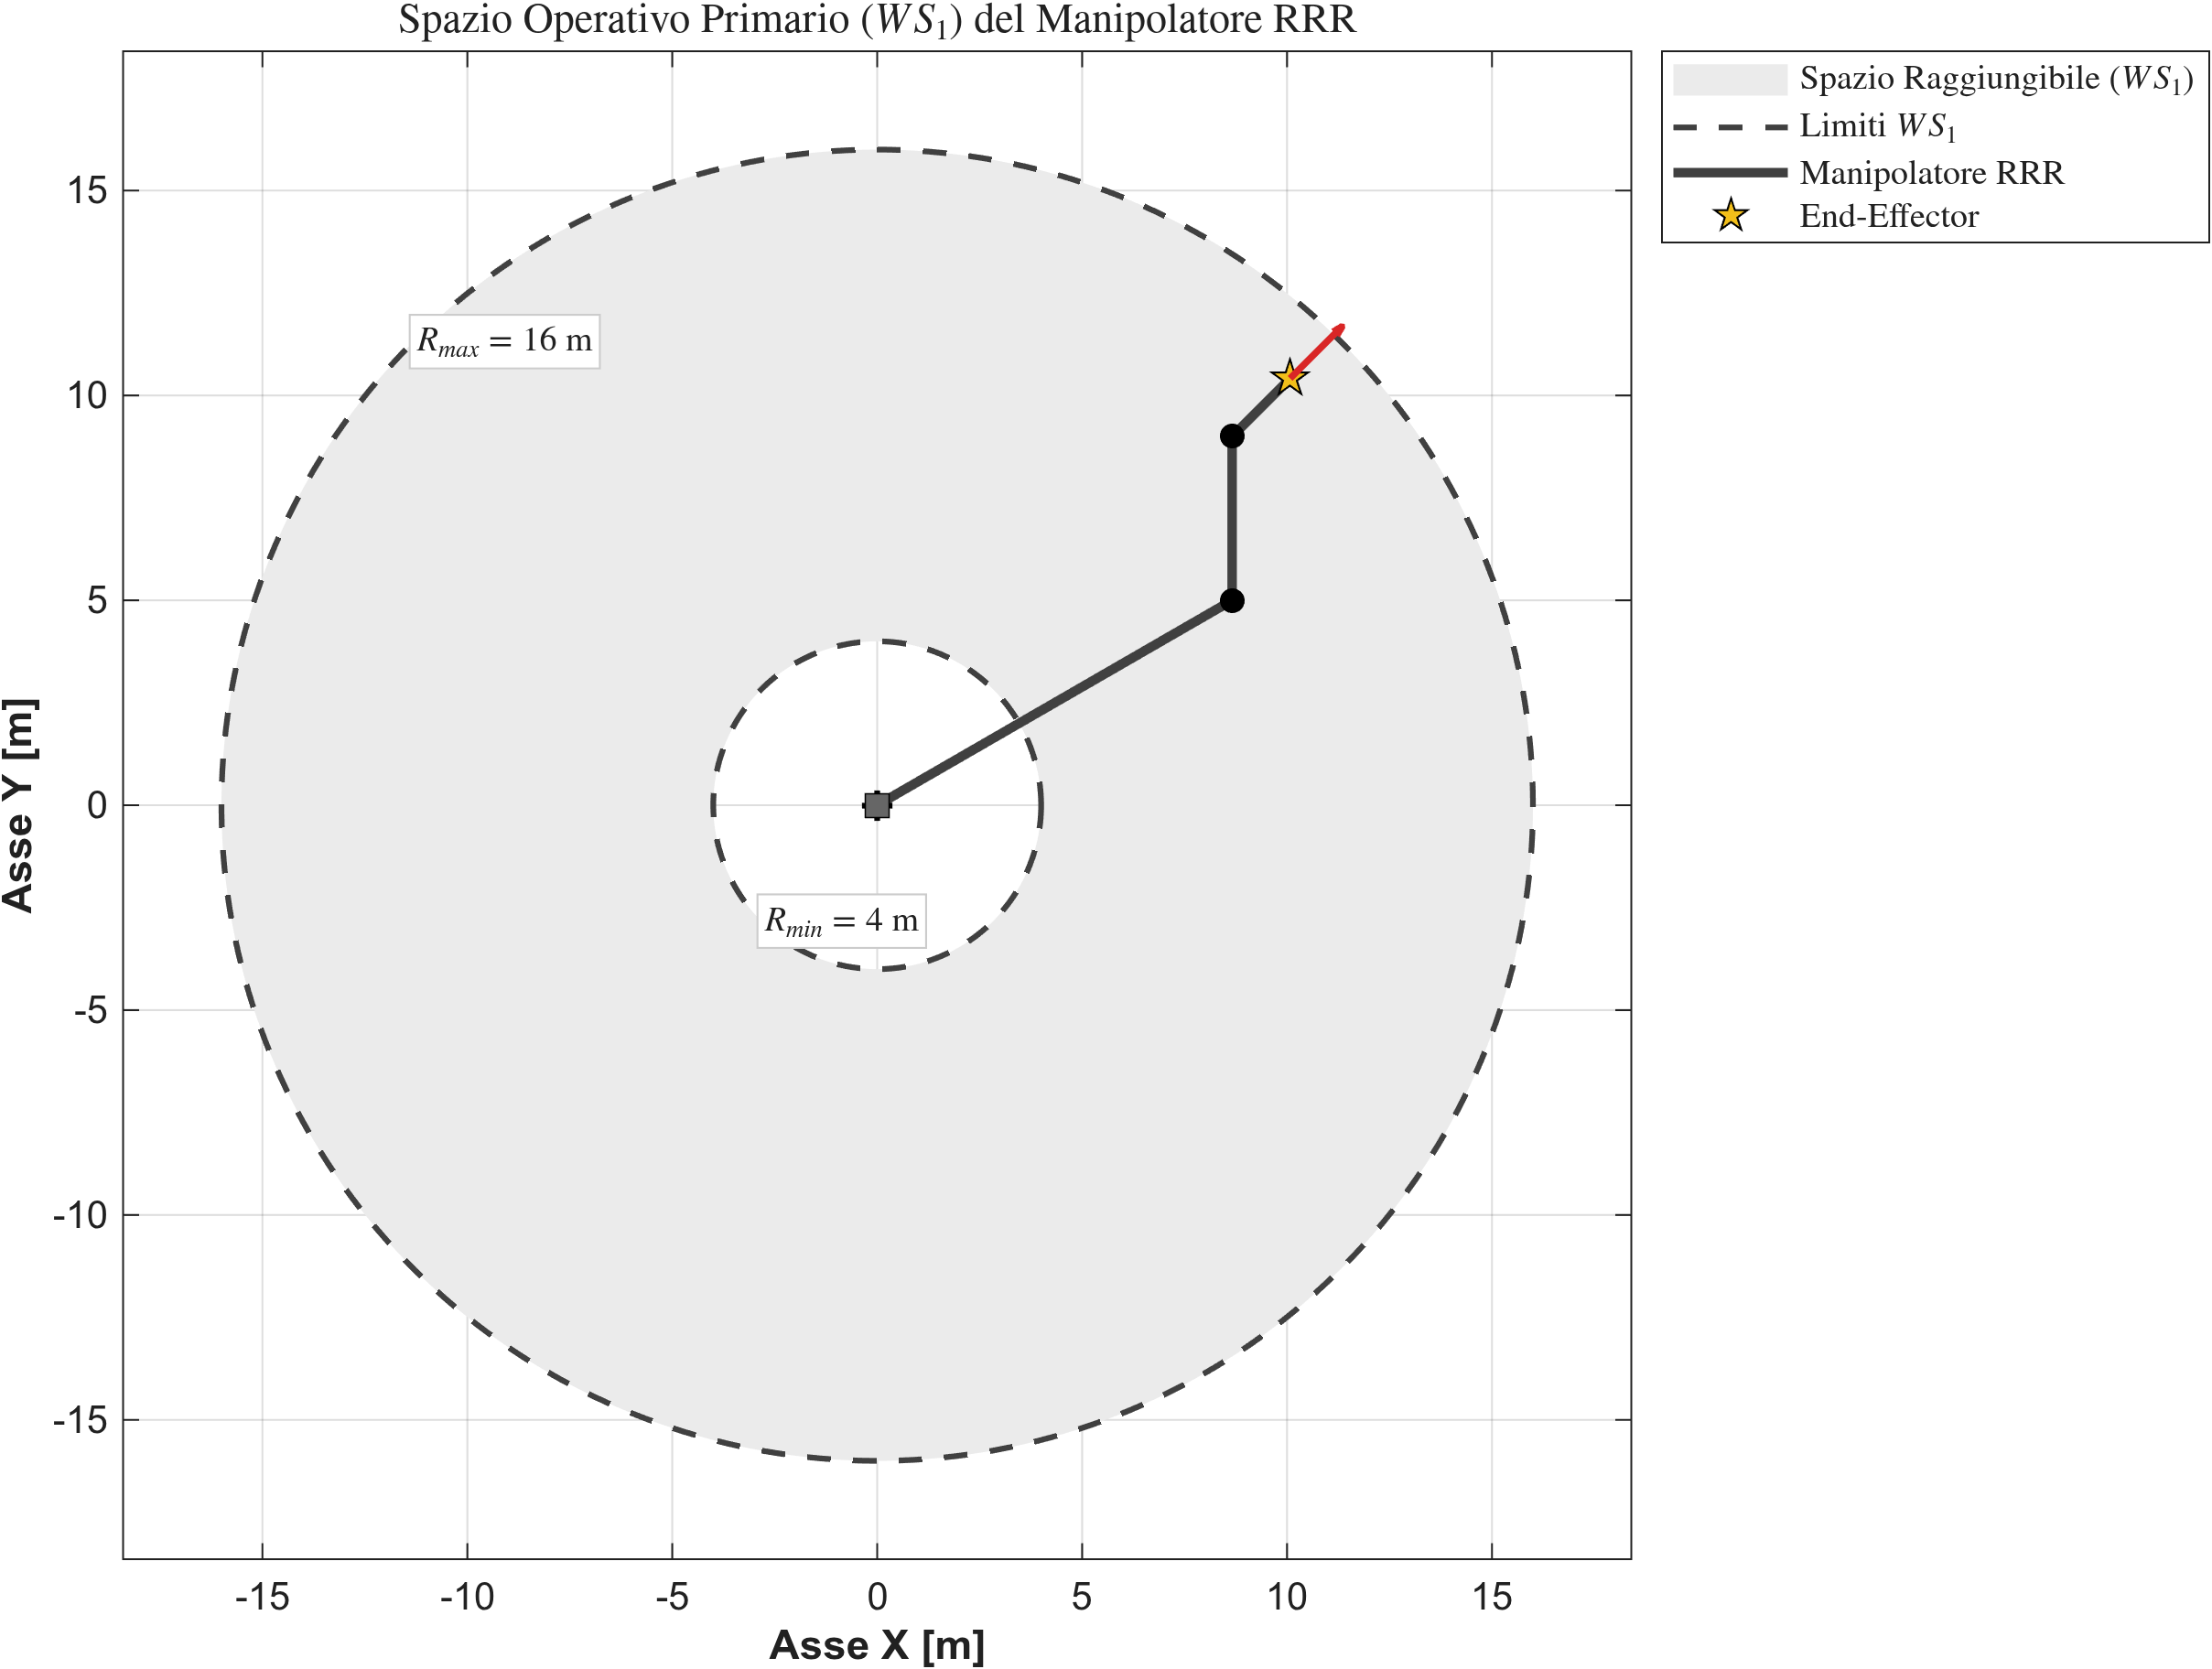
\includegraphics[width=0.65\linewidth]{E5_CinematicaInversaSpaziOperativiManipolatoreRRR_fig1.png}
\end{center}

\begin{par}
\begin{flushleft}
Lo \textit{\textbf{spazio operativo secondario}} è quel sottoinsieme dello spazio primario dove l'end-effector può non solo raggiungere un punto, ma può farlo assumendo qualsiasi orientamento. La capacità di orientarsi liberamente è cruciale in molte applicazioni robotiche.
\end{flushleft}
\end{par}

\begin{par}
\begin{flushleft}
La condizione affinché un punto $P$ appartenga a questo spazio privilegiato è che il cerchio di raggio $l_3$ centrato in $P$ sia interamente contenuto nello spazio di lavoro del polso. Questo garantisce che, per qualsiasi rotazione del terzo braccio, il polso rimanga sempre in una posizione raggiungibile. Analiticamente, la distanza $d$ di un punto $P$ dall'origine deve soddisfare la seguente disuguaglianza:
\end{flushleft}
\end{par}

\[
    |l_1 -l_2 |+l_3 \le d\le l_1 +l_2 -l_3
\]

\begin{par}
\begin{flushleft}
Questa condizione ha senso solo se il raggio minimo è minore o uguale al raggio massimo, ovvero se $|l_1 -l_2 |+l_3 \le l_1 +l_2-l_3$, che si semplifica in $l_3 \le l_2$ (assumendo $l_1 \ge l_2$). Se questa condizione non è rispettata, lo spazio di destrezza è vuoto.
\end{flushleft}
\end{par}

\begin{par}
\begin{flushleft}
Nel caso specifico $l_1 =10,l_2 =4,l_3 =2$, dato che la condizione $l_3 \le l_2$ ($2\le 4$) è soddisfatta, lo spazio di destrezza esiste. I suoi limiti sono:
\end{flushleft}
\end{par}

\begin{itemize}
\setlength{\itemsep}{-1ex}
   \item{\begin{flushleft} Raggio minimo di $WS_2 :\;|10-4|+2=8$ \end{flushleft}}
   \item{\begin{flushleft} Raggio massimo di $WS_2 :\;10+4-2=12$ \end{flushleft}}
\end{itemize}

\begin{par}
\begin{flushleft}
Lo spazio operativo secondario è quindi l'anello definito dalla condizione $8\le d\le 12$. Solo all'interno di questa corona circolare il manipolatore gode della massima destrezza, potendo orientare il suo organo terminale in qualsiasi direzione. Nelle restanti aree dello spazio primario, gli orientamenti possibili sono limitati.
\end{flushleft}
\end{par}

\begin{matlabcode}
% Lo spazio di destrezza esiste solo se il suo raggio massimo è
% maggiore o uguale al suo raggio minimo.
R_min_ws2 = 0;
R_max_ws2 = 0;
if (l1 + l2 - l3) >= (abs(l1-l2) + l3)
    R_min_ws2 = abs(l1 - l2) + l3;
    R_max_ws2 = (l1 + l2) - l3;
end

fprintf('Spazio secondario - raggio interno (R_min_ws2): %.2f\n', R_min_ws2);
fprintf('Spazio secondario - raggio esterno (R_max_ws2): %.2f\n', R_max_ws2);
\end{matlabcode}
\begin{matlaboutput}
Spazio secondario - raggio interno (R_min_ws2): 8.00
Spazio secondario - raggio esterno (R_max_ws2): 12.00
\end{matlaboutput}
\newpage
\begin{matlabcode}
% Figura 2: Spazio operativo primario (WS1) e secondario (WS2)
figure('Name', 'Spazio operativo primario e secondario', 'Color', 'w');
hold on; grid on; box on; axis equal;
xlabel('Asse X [m]', 'FontWeight', 'bold');
ylabel('Asse Y [m]', 'FontWeight', 'bold');

% Coordinate dei cerchi per WS1 (spazio primario) e WS2 (spazio secondario)
theta = linspace(0, 2*pi, 300);
x_ext_ws1 = R_max * cos(theta);      y_ext_ws1 = R_max * sin(theta);
x_int_ws1 = R_min * cos(theta);      y_int_ws1 = R_min * sin(theta);
x_ext_ws2 = R_max_ws2 * cos(theta);  y_ext_ws2 = R_max_ws2 * sin(theta);
x_int_ws2 = R_min_ws2 * cos(theta);  y_int_ws2 = R_min_ws2 * sin(theta);

% Corona WS1 (raggiungibile) e corona WS2 (destrezza)
h_ws1 = fill([x_ext_ws1, fliplr(x_int_ws1)], [y_ext_ws1, fliplr(y_int_ws1)], [0.92, 0.92, 0.92], ...
    'EdgeColor', 'none', 'DisplayName', 'Spazio raggiungibile ($WS_1$)');
h_ws2 = fill([x_ext_ws2, fliplr(x_int_ws2)], [y_ext_ws2, fliplr(y_int_ws2)], [0.80, 0.90, 0.98], ...
    'EdgeColor', 'none', 'DisplayName', 'Spazio di destrezza ($WS_2$)');

% Bordi limite tratteggiati
h_lim_ws1 = plot(x_ext_ws1, y_ext_ws1, '--', 'Color', col_link, 'LineWidth', 1.5, 'DisplayName', 'Limiti $WS_1$');
plot(x_int_ws1, y_int_ws1, '--', 'Color', col_link, 'LineWidth', 1.5, 'HandleVisibility', 'off');
h_lim_ws2 = plot(x_ext_ws2, y_ext_ws2, '--', 'Color', col_blue, 'LineWidth', 1.6, 'DisplayName', 'Limiti $WS_2$');
plot(x_int_ws2, y_int_ws2, '--', 'Color', col_blue, 'LineWidth', 1.6, 'HandleVisibility', 'off');

% Origine assi
plot(0, 0, 'k+', 'MarkerSize', 8, 'LineWidth', 1.5, 'HandleVisibility', 'off');
% Configurazione d'esempio del manipolatore RRR dentro WS2 (destrezza)
q_ex2 = [pi/4, 2*pi/3, -pi/2];
p0 = [0, 0];
p1 = p0 + [l1*cos(q_ex2(1)), l1*sin(q_ex2(1))];
p2 = p1 + [l2*cos(q_ex2(1)+q_ex2(2)), l2*sin(q_ex2(1)+q_ex2(2))];
p3 = p2 + [l3*cos(sum(q_ex2)), l3*sin(sum(q_ex2))];
pts_arm2 = [p0; p1; p2; p3];

h_arm = plot(pts_arm2(:,1), pts_arm2(:,2), '-', 'Color', col_link, 'LineWidth', 2.5, ...
    'DisplayName', 'Manipolatore RRR (in $WS_2$)');
plot(pts_arm2(2:3,1), pts_arm2(2:3,2), 'o', 'MarkerSize', 6, 'MarkerFaceColor', 'k', 'MarkerEdgeColor', 'k', ...
    'HandleVisibility', 'off');
plot(p0(1), p0(2), 's', 'MarkerSize', 8, 'MarkerFaceColor', [0.4, 0.4, 0.4], 'MarkerEdgeColor', 'k', ...
    'HandleVisibility', 'off');
h_ee = plot(p3(1), p3(2), 'p', 'MarkerSize', 10, 'MarkerFaceColor', [0.95, 0.75, 0.10], ...
    'MarkerEdgeColor', 'k', 'DisplayName', 'End-effector');
quiver(p3(1), p3(2), 1.8*cos(sum(q_ex2)), 1.8*sin(sum(q_ex2)), 0, 'Color', col_red, 'LineWidth', 1.8, 'MaxHeadSize', 0.6, 'HandleVisibility', 'off');

% Annotazioni raggi WS2 (posizionate nel II/III quadrante, lontano dal braccio)
ang_ws2_in = -3*pi/4;  ang_ws2_out = 3*pi/4;
text(R_min_ws2*cos(ang_ws2_in), R_min_ws2*sin(ang_ws2_in), sprintf('$R_{min,WS2} = %.0f$ m', R_min_ws2), ...
    'Interpreter', 'latex', 'FontSize', 9, 'FontWeight', 'bold', 'BackgroundColor', [1 1 1], ...
    'EdgeColor', [0.8 0.8 0.8], 'Margin', 1);
text(R_max_ws2*cos(ang_ws2_out), R_max_ws2*sin(ang_ws2_out), sprintf('$R_{max,WS2} = %.0f$ m', R_max_ws2), ...
    'Interpreter', 'latex', 'FontSize', 9, 'FontWeight', 'bold','BackgroundColor', [1 1 1], ...
    'EdgeColor', [0.8 0.8 0.8], 'Margin', 1);

title('Spazio operativo primario ($WS_1$) e secondario ($WS_2$)', 'Interpreter', 'latex', 'FontSize', 11, ...
    'FontWeight', 'bold');
legend([h_ws1, h_ws2, h_lim_ws1, h_lim_ws2, h_arm, h_ee], 'Interpreter', 'latex', 'Location', 'bestoutside');
lim = R_max * 1.15;
xlim([-lim, lim]); ylim([-lim, lim]);
hold off;
\end{matlabcode}
\begin{center}
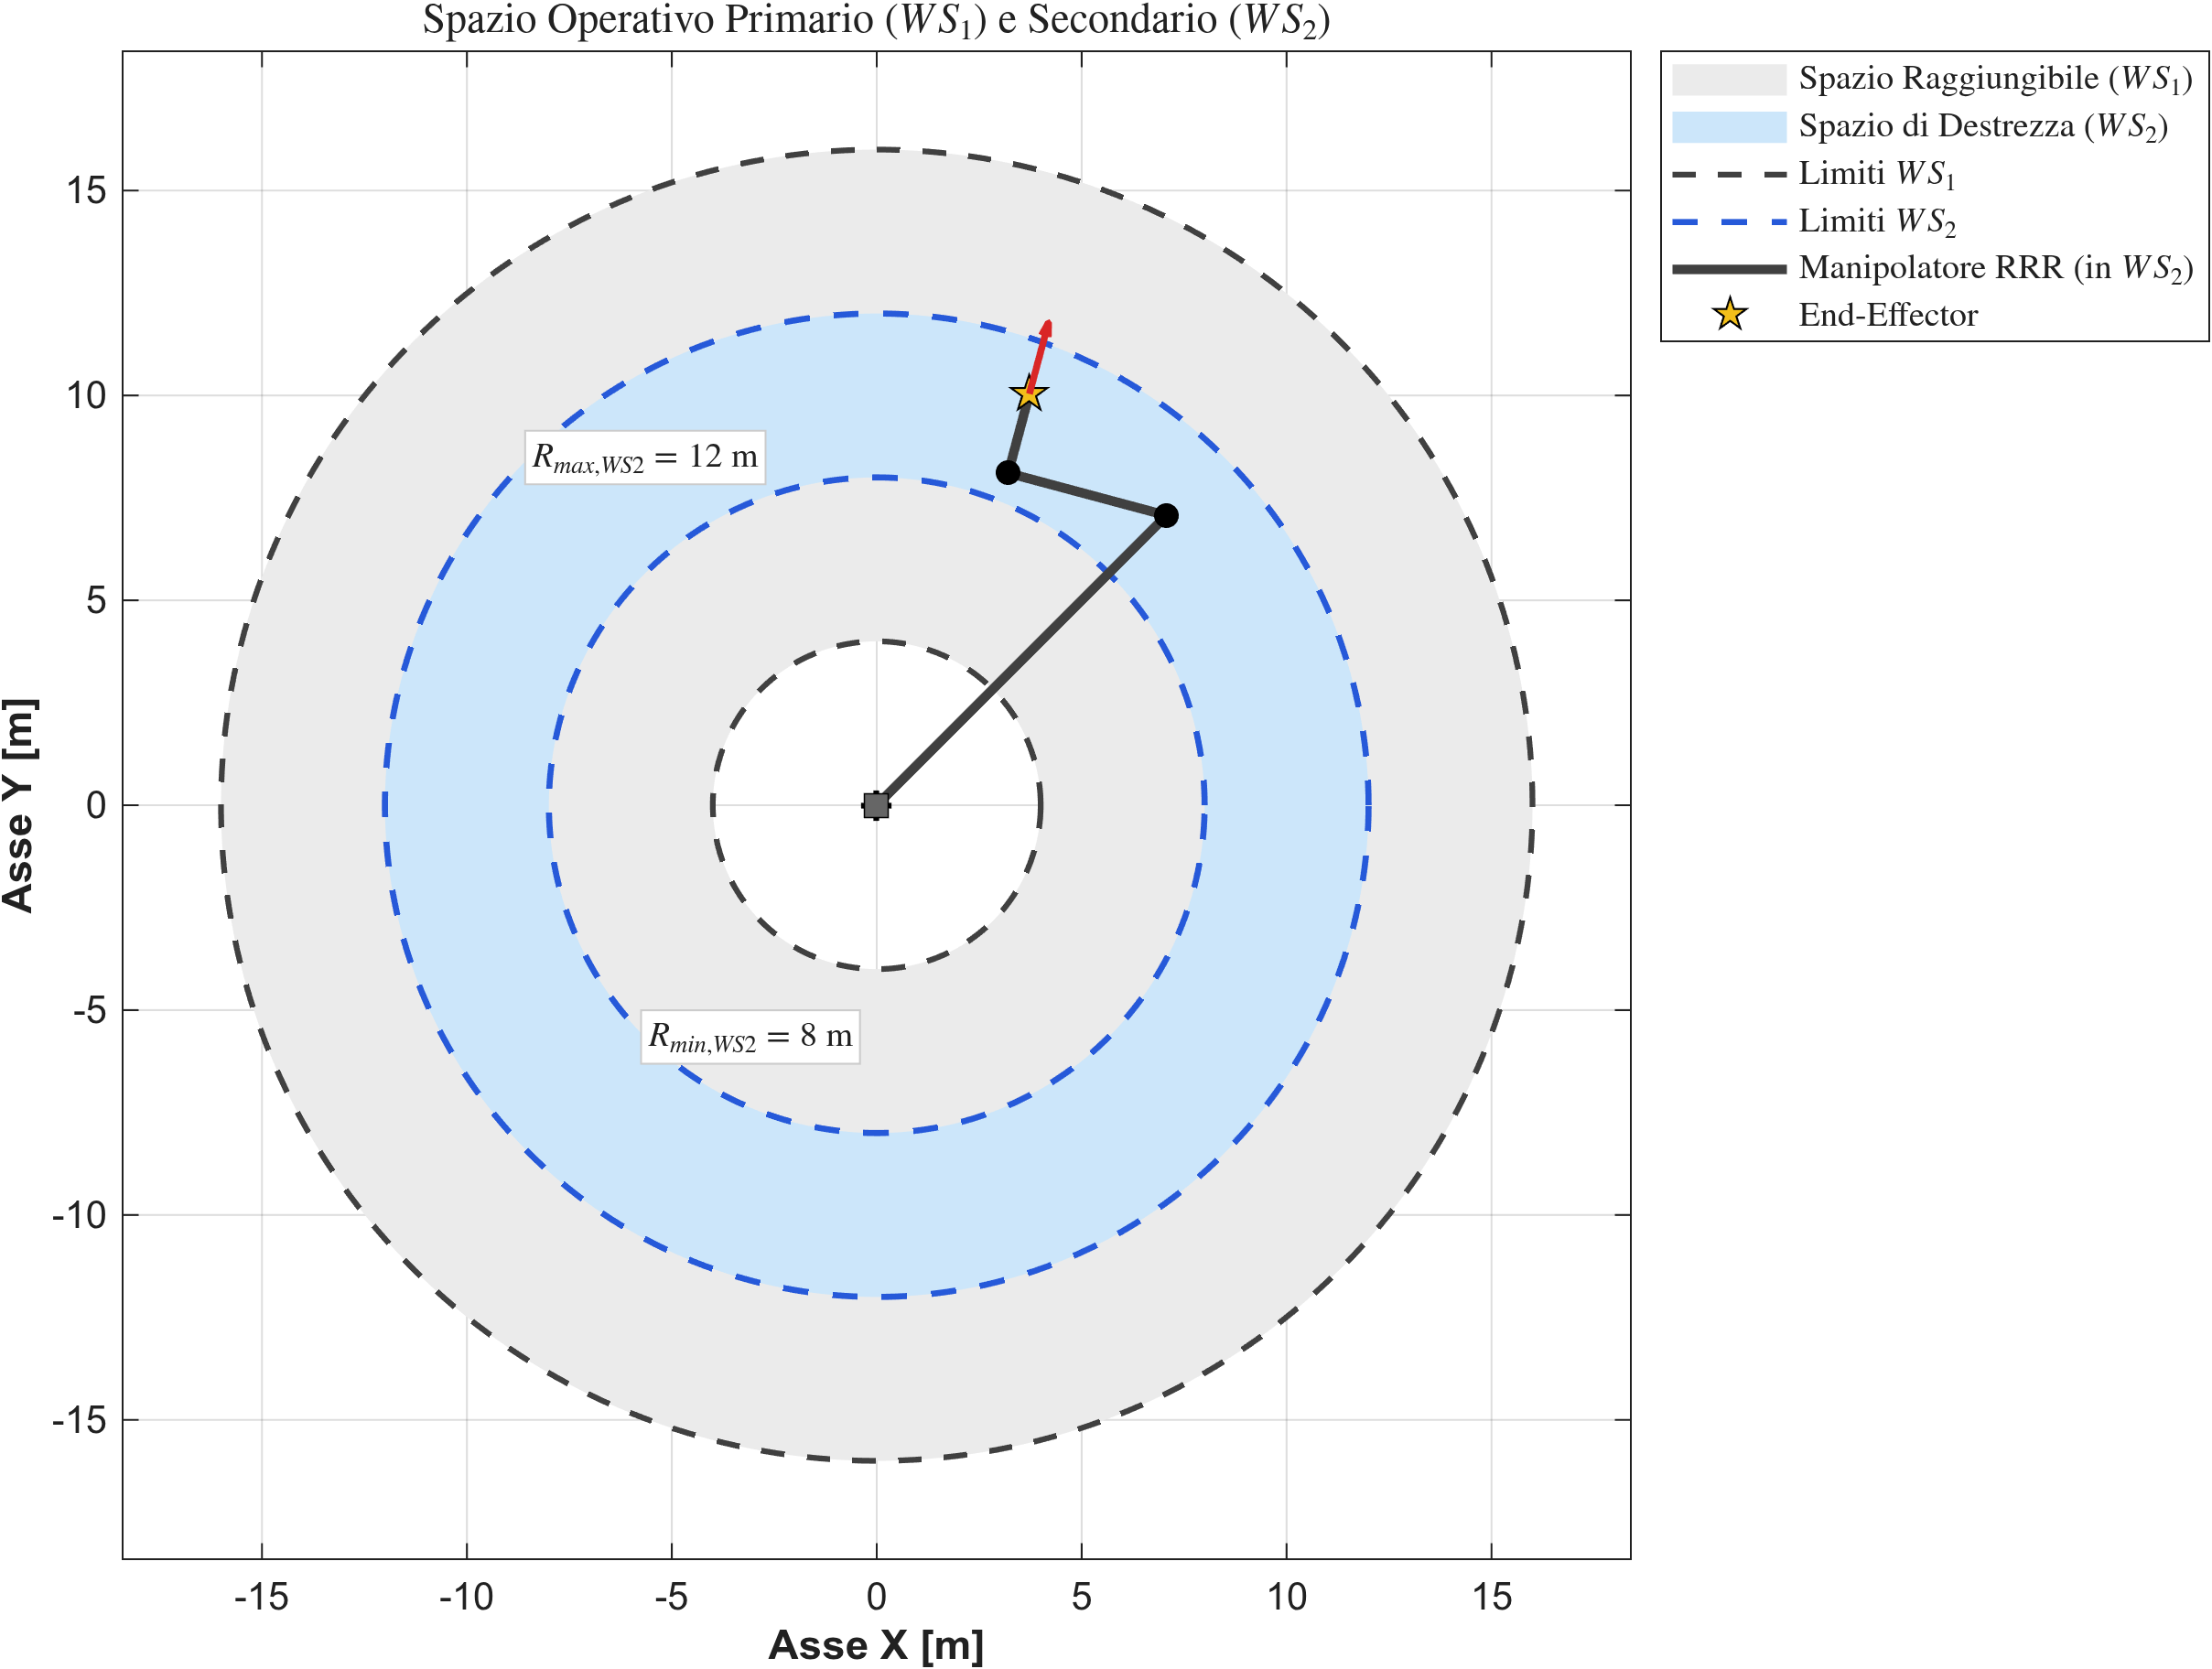
\includegraphics[width=0.9\linewidth]{E5_CinematicaInversaSpaziOperativiManipolatoreRRR_fig2.png}
\end{center}

\end{document}
